\documentclass[11pt,a4paper]{article}

\usepackage[margin=25mm]{geometry}
\usepackage{amsmath}
\usepackage{booktabs}
\usepackage{float}
\usepackage{graphicx}
\usepackage[hidelinks]{hyperref}
\usepackage{microtype}

\graphicspath{{../results/figures/}}
\setlength{\emergencystretch}{2em}

\title{Comparative Evaluation of the SystemDS PowerTransformer}
\author{Wenliang Cao}
\date{August 2026}

\begin{document}

\maketitle

\begin{abstract}
This report evaluates the Apache SystemDS PowerTransformer against no scaling,
standard scaling, and robust scaling on regression, classification, and
clustering tasks. The implementation supports Yeo--Johnson and Box--Cox
transformations, estimates one parameter per feature, standardizes transformed
features, and reuses fitted parameters on unseen data. Nine public tabular
datasets are evaluated with five fixed random seeds. Distance-based downstream
estimators are held constant to isolate the effect of preprocessing. A power
transformation ranks first or ties for first on four of the nine datasets, with
the strongest gain on the highly skewed Wholesale Customers clustering task.
The results also show that no preprocessing method dominates every dataset.
\end{abstract}

\tableofcontents
\newpage

\section{Scope}

The experiment addresses two questions. First, does a fitted power
transformation improve distance-based prediction or clustering compared with
common scaling baselines? Second, what preprocessing cost accompanies that
change? The evaluation is comparative rather than a test of universal
superiority. All methods use the same data splits, random seeds, and downstream
estimator parameters.

\section{Implementation under test}

SystemDS performs every fitted transformation. The training operation returns
the transformed matrix and the fitted parameters:

\begin{verbatim}
[Y, lambdas, means, scales] = powerTransform(
    X, method="yeo-johnson", standardize=TRUE)
\end{verbatim}

The apply operation reuses those parameters without fitting on test data:

\begin{verbatim}
Ytest = powerTransformApply(
    Xtest, lambdas, means, scales, method="yeo-johnson")
\end{verbatim}

Yeo--Johnson is the default because it is defined over the real line. Box--Cox
is available through \texttt{method="box-cox"} and requires strictly positive
features. With standardization enabled, the fitted means and scales are derived
from the transformed training matrix and reused by the apply operation.

For a positive value $x$, the Box--Cox family is

\begin{equation}
T_{\lambda}(x)=
\begin{cases}
(x^{\lambda}-1)/\lambda, & \lambda \neq 0,\\
\log(x), & \lambda=0.
\end{cases}
\end{equation}

The Yeo--Johnson family extends the same principle to zero and negative values.
SystemDS estimates each feature's parameter by maximizing the profile
log-likelihood with Brent optimization.

\section{Experimental methodology}

\subsection{Preprocessing methods}

The comparison contains five methods: no scaling, standard scaling, robust
scaling based on the median and interquartile range, standardized Yeo--Johnson,
and standardized Box--Cox. No offset is added to make Box--Cox applicable.
Two Abalone records with zero height are excluded according to the frozen data
preparation rule; all other datasets retain their full row set.

\subsection{Datasets}

The matrix contains two compact core datasets and one preselected skew-focused
dataset for each task. The skew-focused configuration was frozen before the
downstream results were inspected. Its selection requirements are public
tabular data, numeric features without missing values, median absolute feature
skewness above 2.0, and at least 5,000 rows for supervised tasks.

\input{generated/datasets.tex}

\subsection{Downstream estimators}

Regression uses \texttt{KNeighborsRegressor}; classification uses
\texttt{KNeighborsClassifier}. Both use five neighbors, uniform weights,
Euclidean distance, and one execution thread. Clustering uses K-means with the
known class count, 20 initializations, and the experiment seed as
\texttt{random\_state}. These models are sensitive to feature geometry, which
makes them suitable for comparing preprocessing methods. No estimator or
method-specific hyperparameter tuning is performed.

\subsection{Splits, seeds, and leakage control}

The fixed seeds are 13, 37, 73, 101, and 149. Regression and classification use
80/20 train/test splits. Classification splits are stratified. Parkinsons
Telemonitoring uses a group shuffle split so that recordings from the same
subject cannot occur in both training and test data. Each transformer is fitted
only on the training features and applied to the corresponding test features.
Clustering uses the full dataset for each seed.

\subsection{Metrics}

Regression is ranked by root mean squared error (RMSE), with $R^2$ as a
secondary metric. Classification is ranked by macro-averaged F1, with accuracy
as a secondary metric. Clustering is ranked by adjusted Rand index (ARI), with
silhouette score as a secondary metric. RMSE is minimized; the other metrics
are maximized. Tables report the mean and sample standard deviation over five
runs.

\section{Results}

\subsection{Regression}

\input{generated/regression-primary.tex}

Yeo--Johnson obtains the lowest mean RMSE on California Housing: 0.6114 versus
0.6486 for standard scaling, a 5.74\% reduction. No scaling leads on Abalone,
while robust scaling leads on Parkinsons Telemonitoring. The result is therefore
dataset-dependent even within one task and estimator.

\begin{figure}[H]
\centering
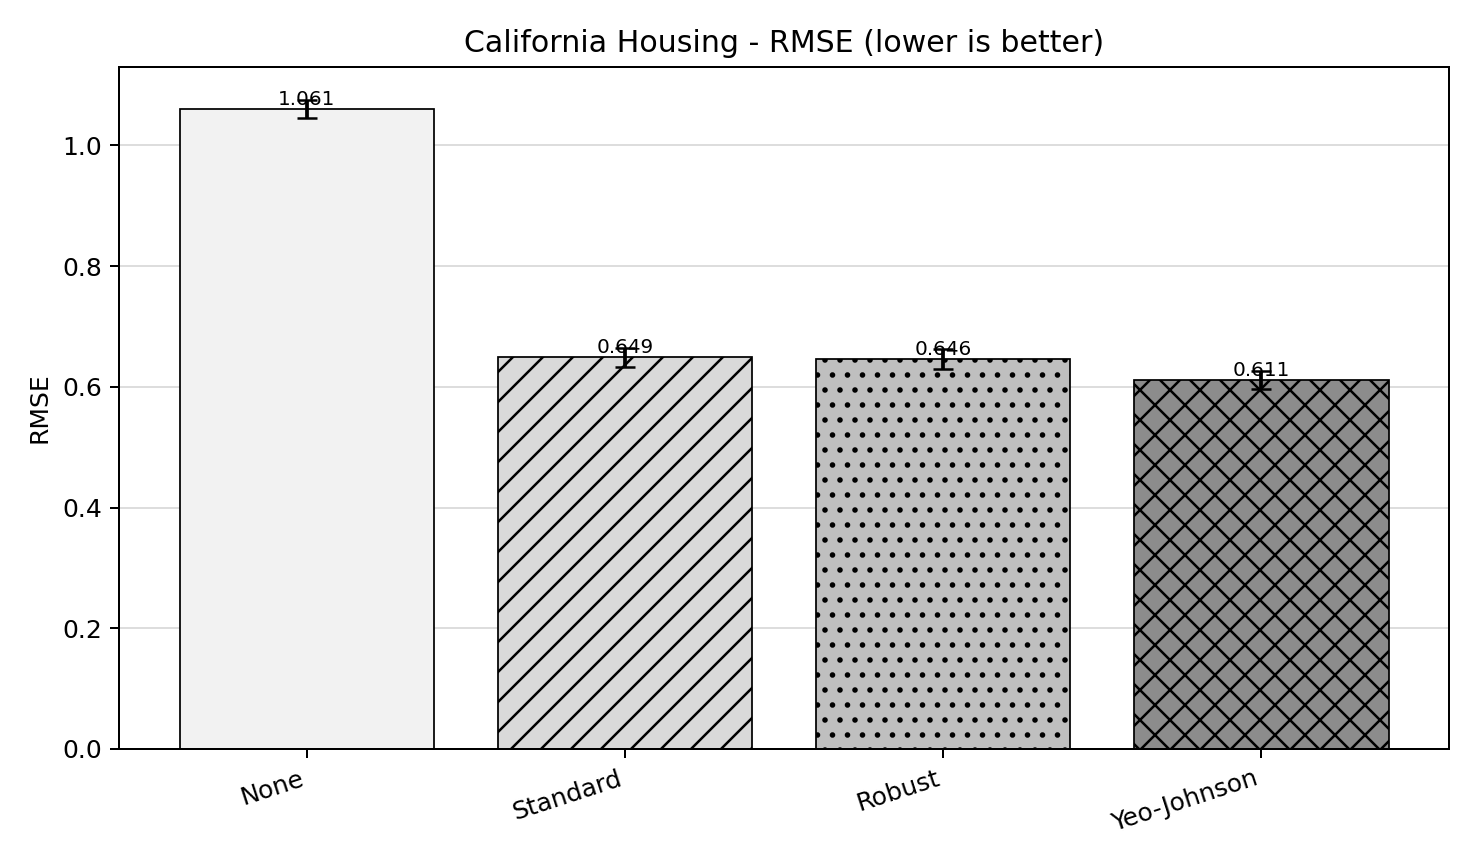
\includegraphics[width=0.86\textwidth]{california_housing-rmse.png}
\caption{California Housing regression performance. Error bars show one sample standard deviation.}
\end{figure}

\begin{figure}[H]
\centering
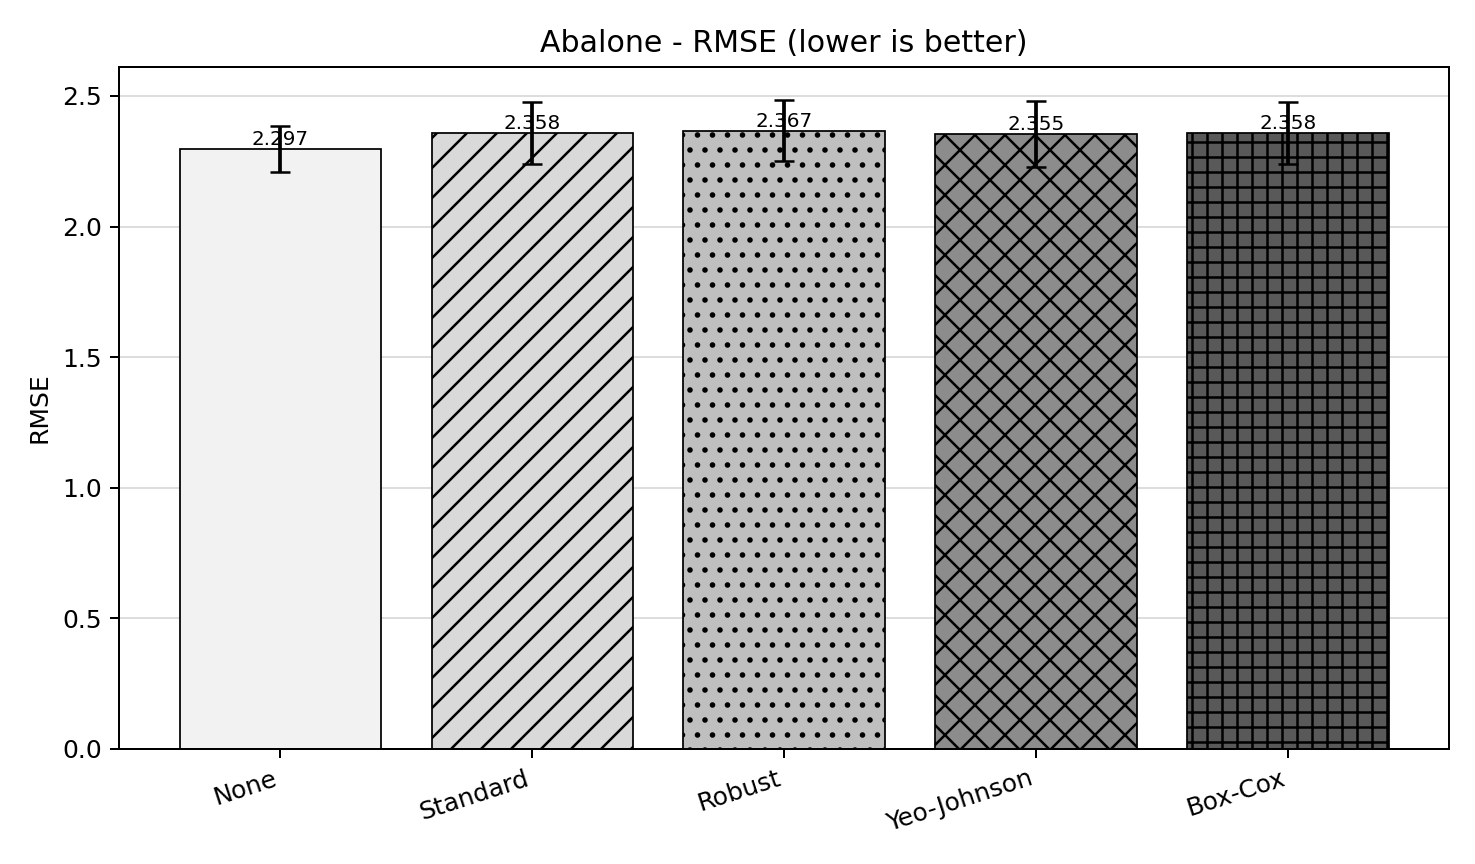
\includegraphics[width=0.48\textwidth]{abalone-rmse.png}\hfill
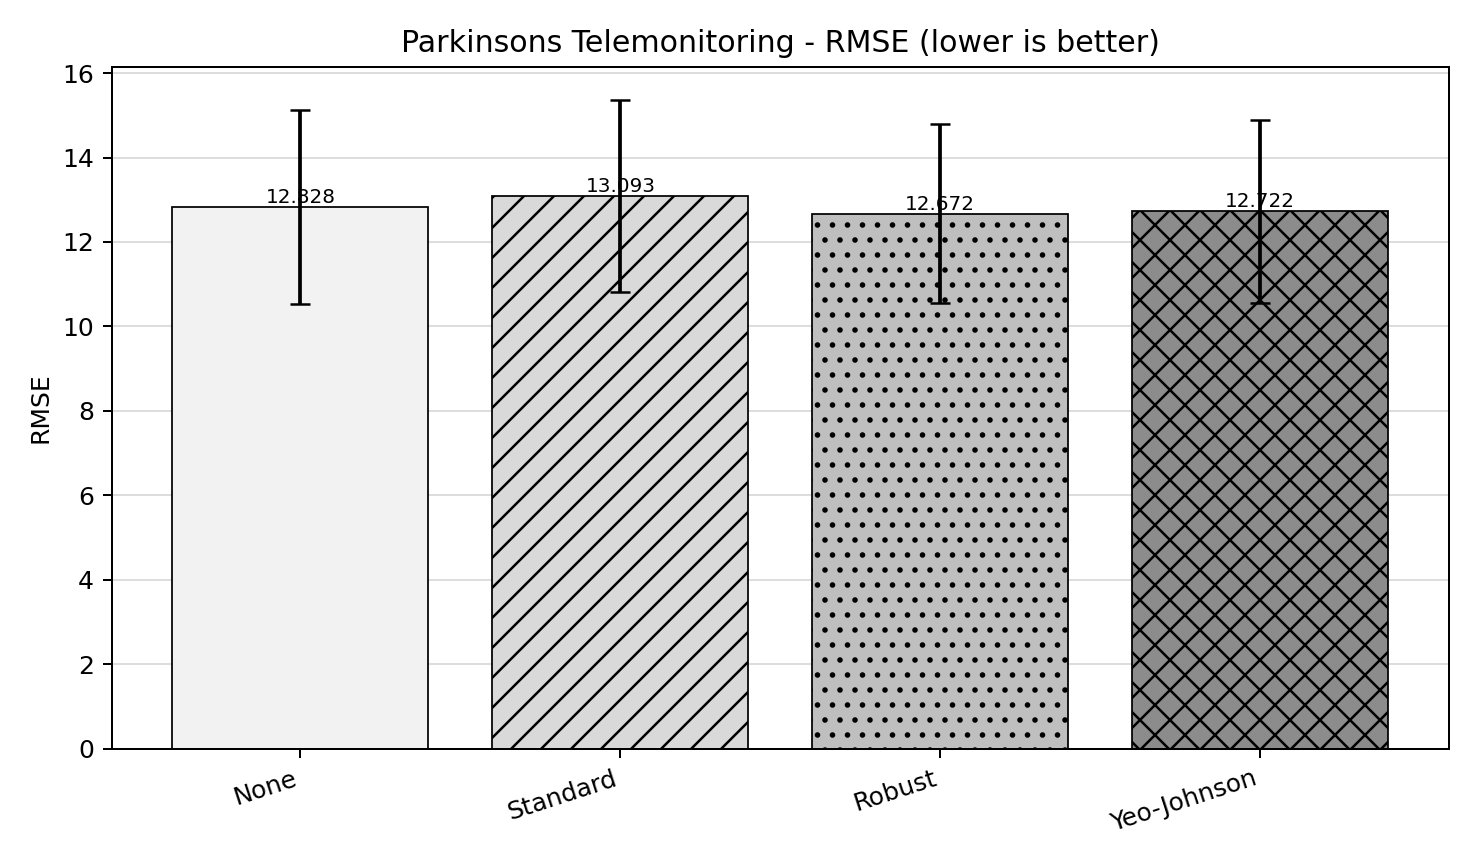
\includegraphics[width=0.48\textwidth]{parkinsons_telemonitoring-rmse.png}
\caption{Abalone and Parkinsons Telemonitoring regression performance.}
\end{figure}

\subsection{Classification}

\input{generated/classification-primary.tex}

Yeo--Johnson leads on Breast Cancer Wisconsin with a mean macro-F1 of 0.9618.
Standard scaling leads on Wine, and robust scaling leads on HTRU2. The HTRU2
result is close: robust scaling scores 0.9339 and Yeo--Johnson scores 0.9327.

\begin{figure}[H]
\centering
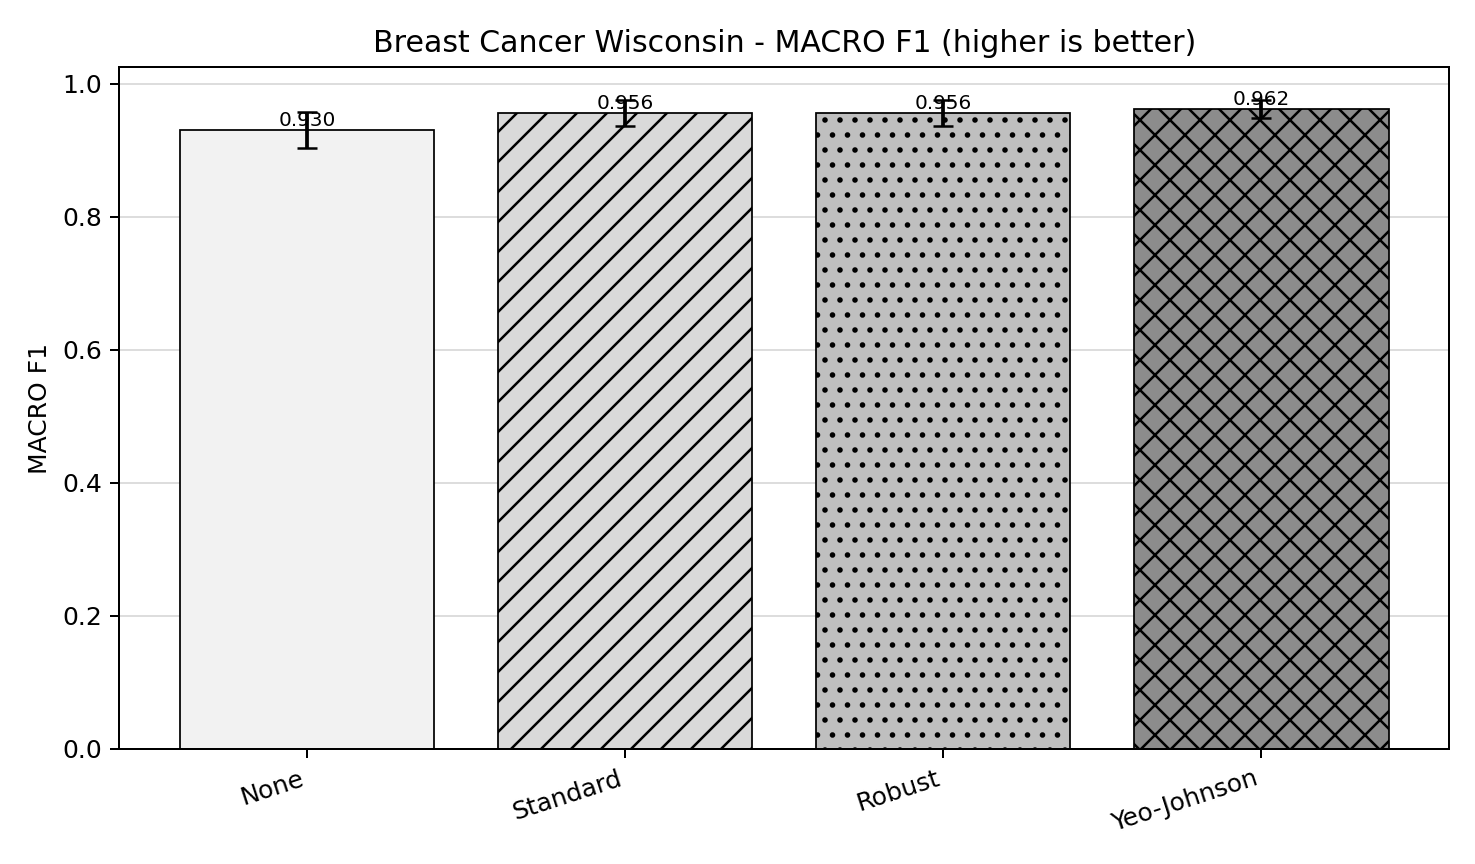
\includegraphics[width=0.48\textwidth]{breast_cancer-macro_f1.png}\hfill
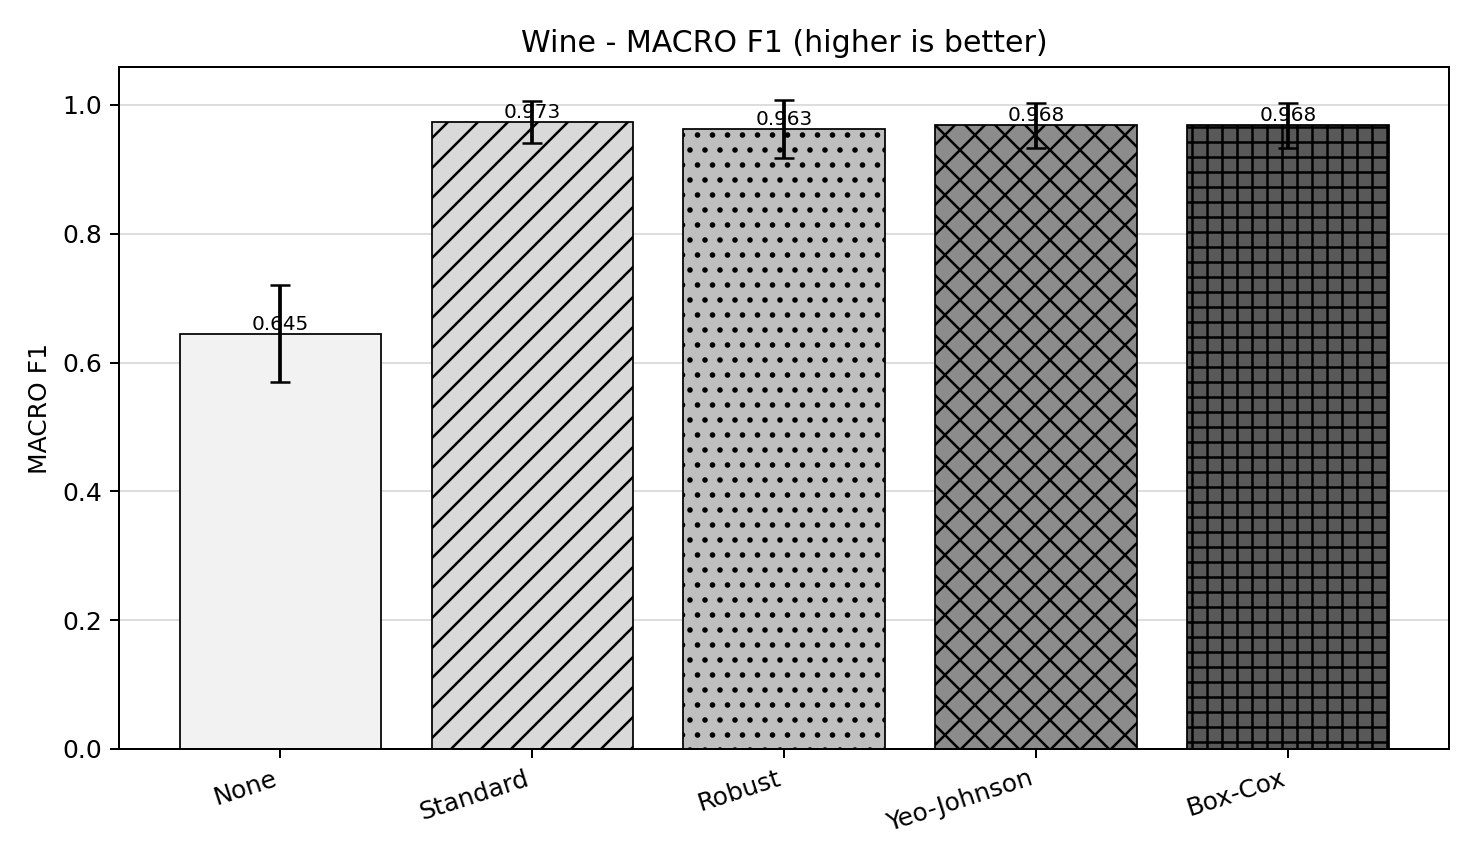
\includegraphics[width=0.48\textwidth]{wine-macro_f1.png}
\caption{Breast Cancer Wisconsin and Wine classification performance.}
\end{figure}

\begin{figure}[H]
\centering
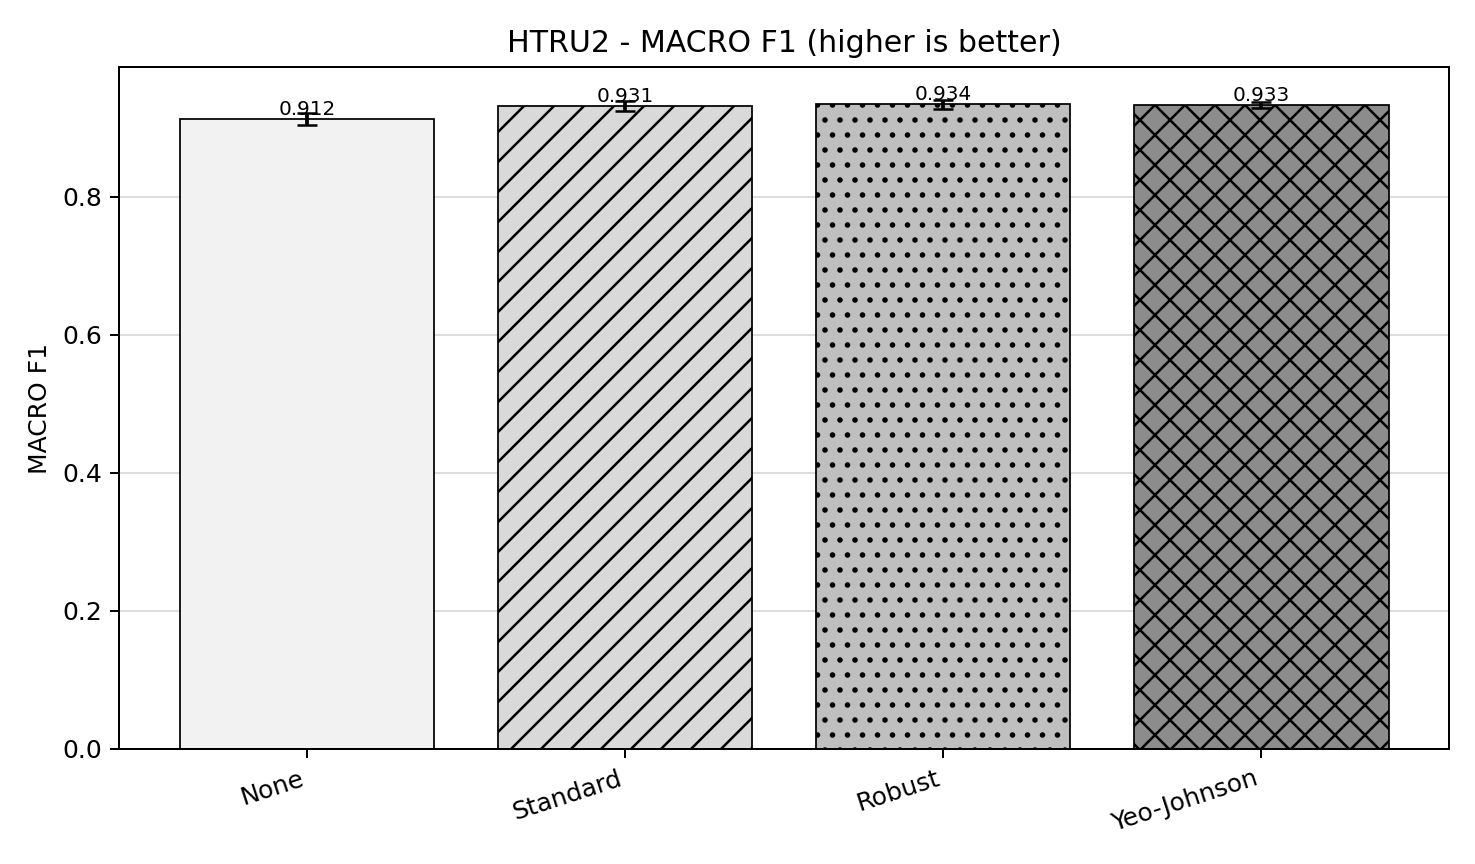
\includegraphics[width=0.72\textwidth]{htru2-macro_f1.png}
\caption{HTRU2 classification performance.}
\end{figure}

\subsection{Clustering}

\input{generated/clustering-primary.tex}

No scaling leads on Iris. Yeo--Johnson and Box--Cox tie on Seeds at the reported
precision. On Wholesale Customers, Box--Cox reaches an ARI of 0.5330 and
Yeo--Johnson reaches 0.5264, compared with 0.1873 for standard scaling. This is
the clearest case in which reducing extreme right skew changes the K-means
geometry in a useful way.

\begin{figure}[H]
\centering
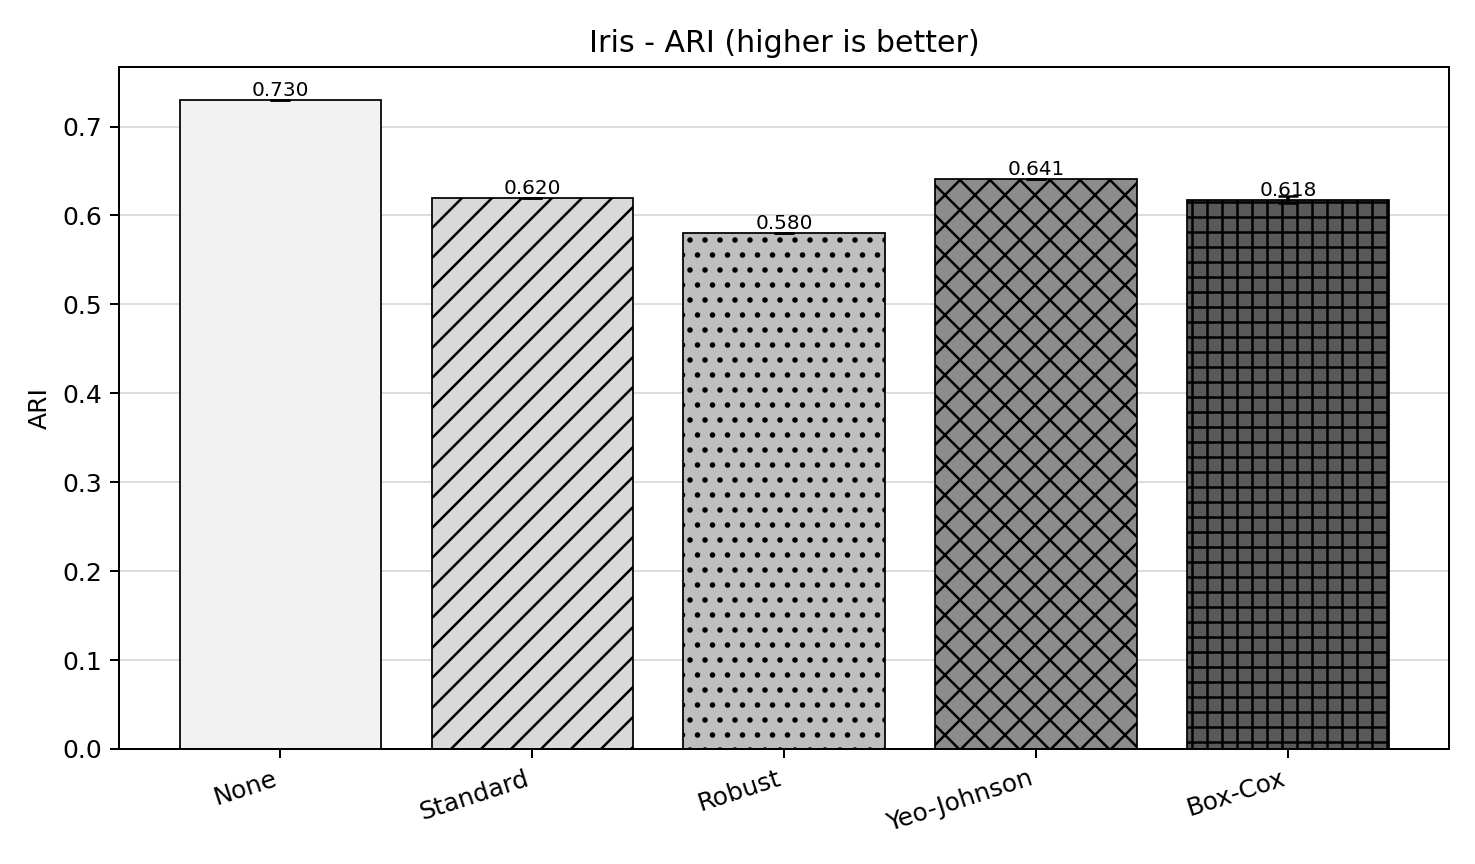
\includegraphics[width=0.48\textwidth]{iris-ari.png}\hfill
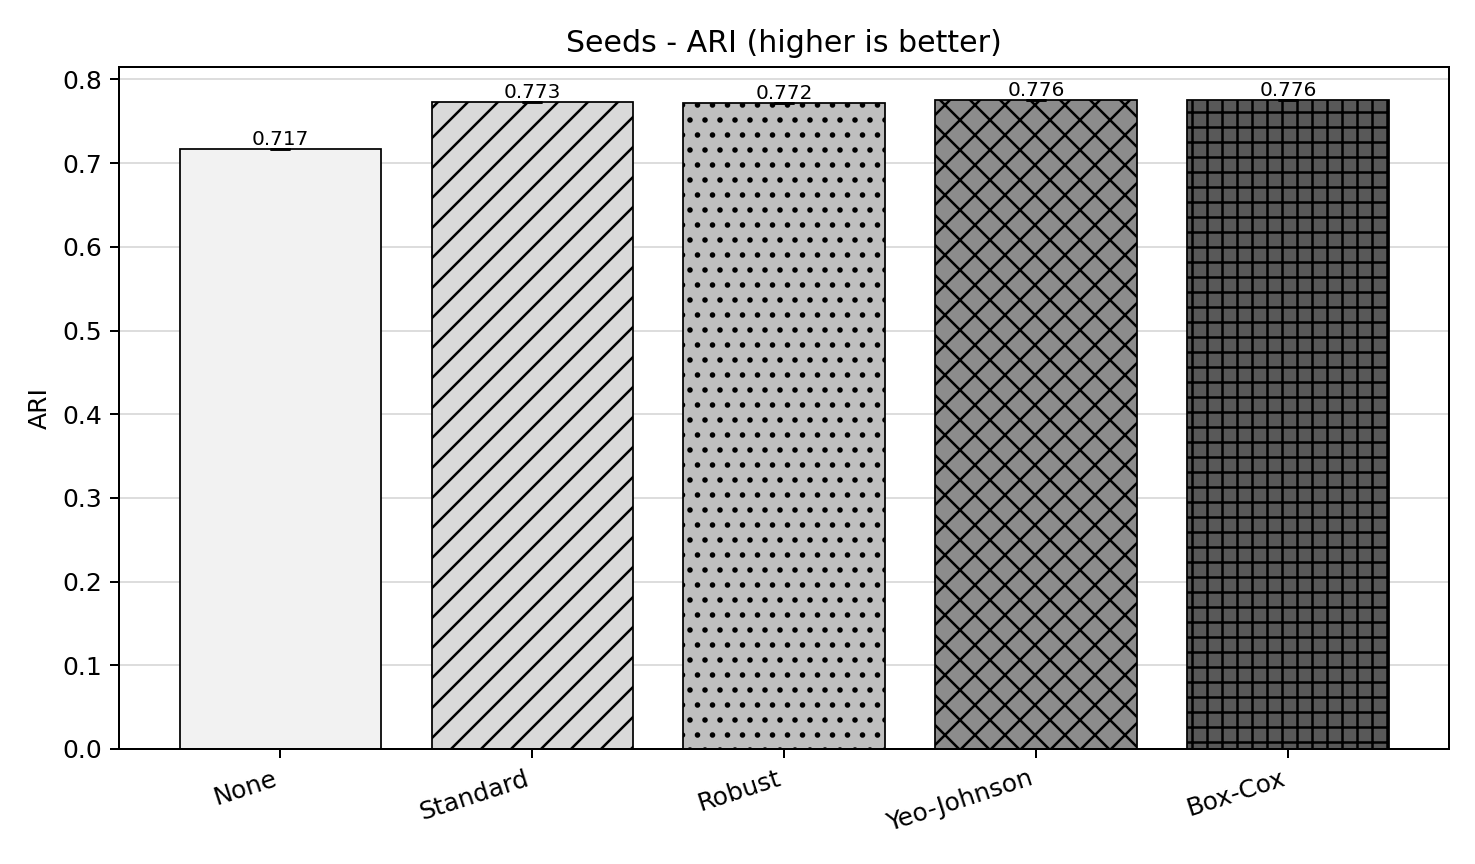
\includegraphics[width=0.48\textwidth]{seeds-ari.png}
\caption{Iris and Seeds clustering performance.}
\end{figure}

\begin{figure}[H]
\centering
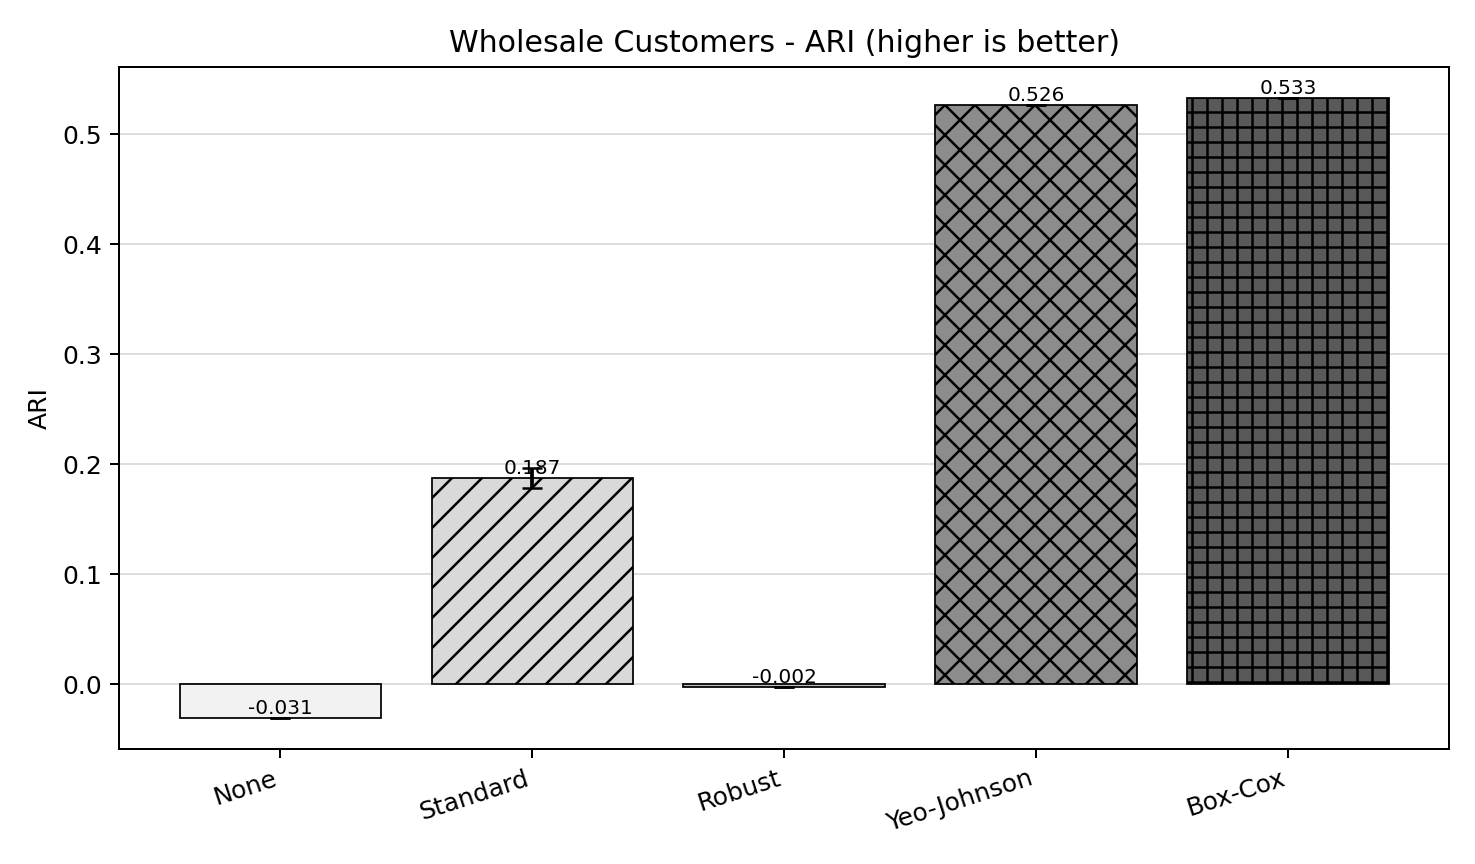
\includegraphics[width=0.72\textwidth]{wholesale_customers-ari.png}
\caption{Wholesale Customers clustering performance.}
\end{figure}

\subsection{Preprocessing time}

\input{generated/runtime.tex}

\begin{figure}[H]
\centering
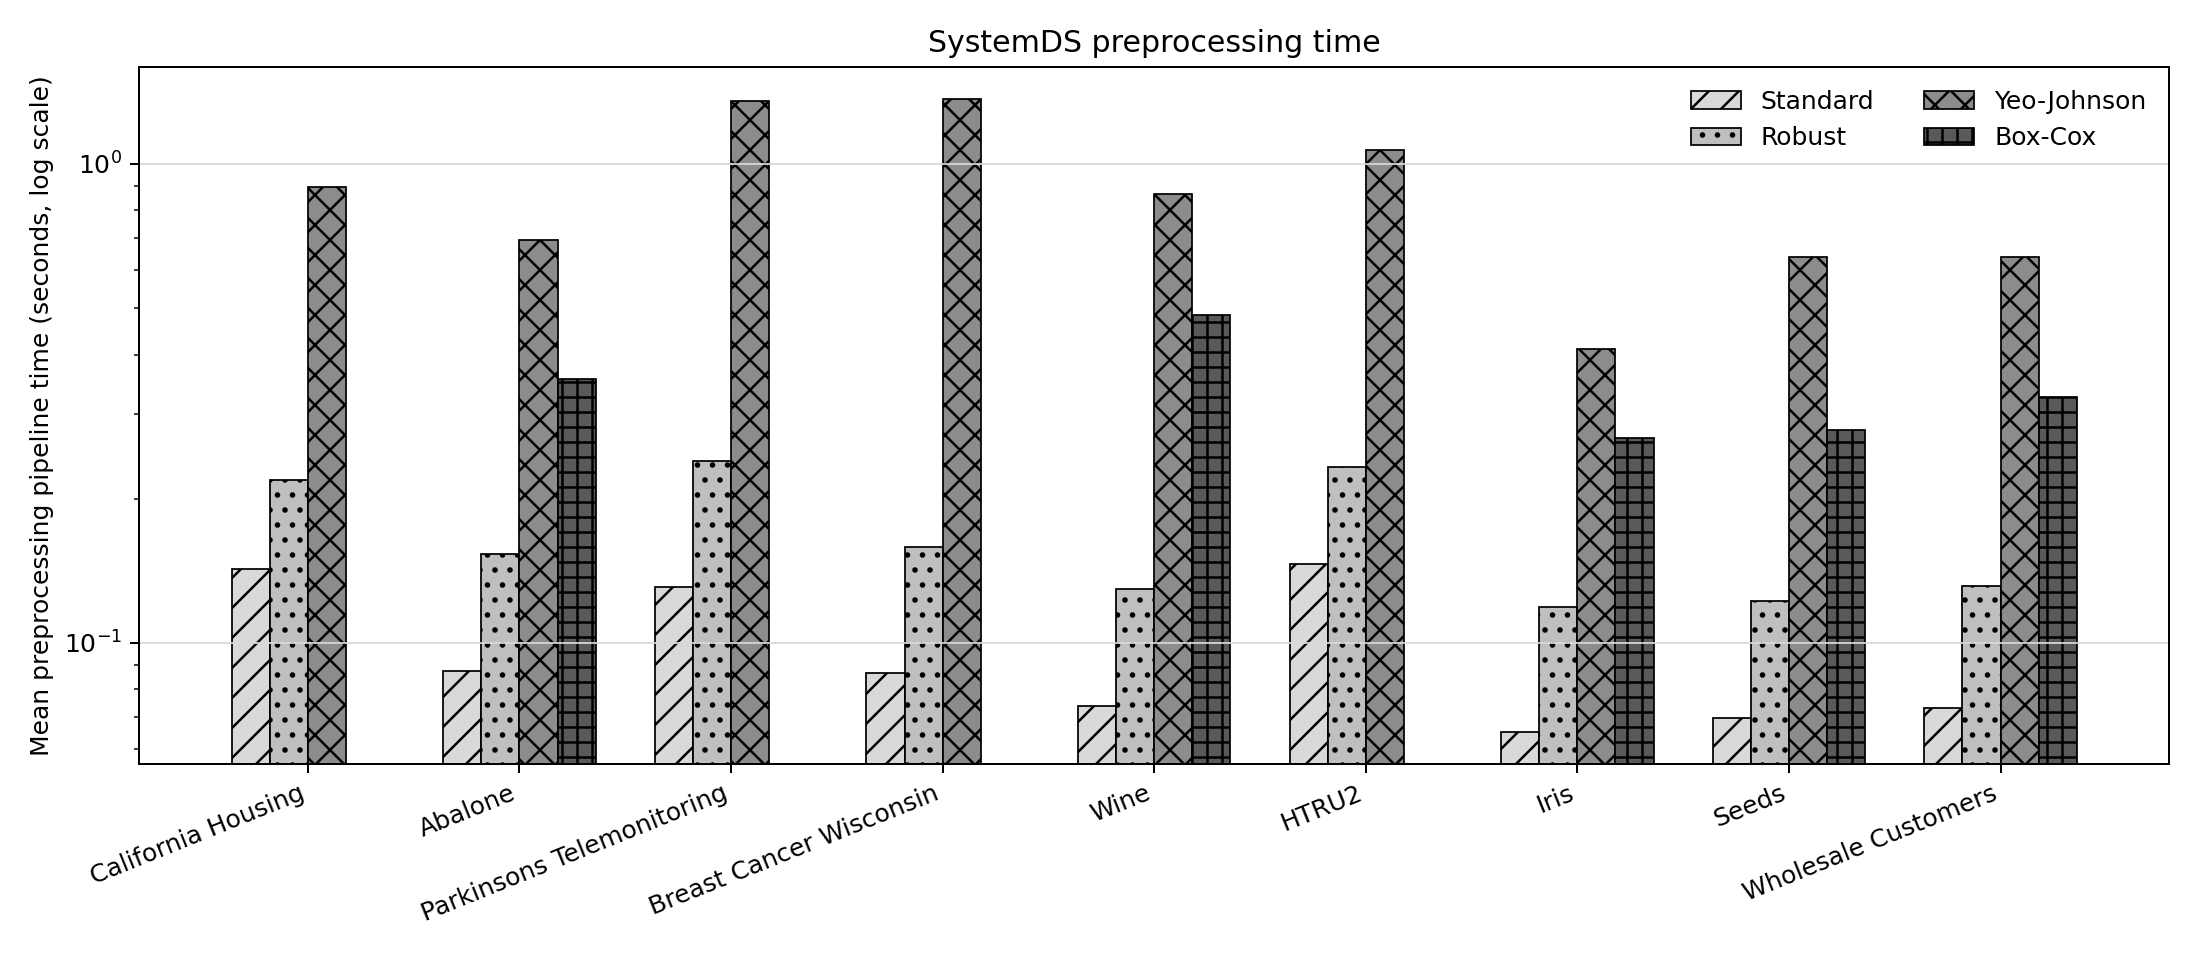
\includegraphics[width=\textwidth]{preprocessing-runtime.png}
\caption{Mean SystemDS preprocessing pipeline time on a logarithmic scale.}
\end{figure}

Power transformations are slower than standard and robust scaling because every
feature requires repeated likelihood evaluations during parameter estimation.
The recorded time covers fit, apply, and transformed-matrix writes; it is a
pipeline measurement rather than an isolated optimizer microbenchmark.

\section{Secondary metrics}

The secondary metrics are reported to prevent conclusions from depending on a
single score. Internal and external clustering criteria can disagree: silhouette
measures Euclidean separation, whereas ARI compares assignments with reference
labels.

\input{generated/regression-secondary.tex}
\input{generated/classification-secondary.tex}
\input{generated/clustering-secondary.tex}

\section{Discussion}

A power transformation ranks first or ties for first on four datasets:
California Housing, Breast Cancer Wisconsin, Seeds, and Wholesale Customers.
The benefit is largest when nonlinear marginal skew materially distorts the
distance geometry, as in Wholesale Customers. Mildly skewed or already
well-separated datasets do not necessarily improve. This is expected: a power
transformation changes marginal feature distributions but does not optimize the
downstream task directly.

Yeo--Johnson remains the general default because it accepts positive, zero, and
negative values. Box--Cox is a useful explicit option for strictly positive
features and leads on Wholesale Customers. The results support providing both
methods while avoiding a claim that either method should win on every dataset.

\section{Limitations}

The evaluation uses three datasets per task, five seeds, and one fixed estimator
family per task. It is not a universal benchmark. The skew-focused extension
contains one preselected dataset per task. No statistical significance test,
cross-validation study, missing-value study, inverse transformation, or
method-specific hyperparameter search is included. Runtime measurements come
from one Apple Silicon machine and small tabular datasets. Transformations run
in SystemDS; downstream estimators and metrics run in scikit-learn.

\end{document}
